\section{Experimental Evaluation}
\label{sec:evaluation}

To evaluate the \sys{} framework, we
first introduce an experimental setup (\autoref{sec:exp_setup}). Then, we
compare our algorithms against the state of the art for event query
discovery (\autoref{sec:exp_sota}). Finally, we evaluate the sensitivity of
our algorithms with respect to the characteristics of a stream database
(\autoref{sec:exp_sensitity}), before studying the effectiveness of our
strategies to guide the application of discovery algorithms
(\autoref{sec:exp_guidance}).

\subsection{Experimental Setup}
\label{sec:exp_setup}


\sstitle{Datasets}
We leverage both real-world and synthetic data to
evaluate our algorithms.
Specifically, we rely on NASDAQ stock trade events~\cite{eodata}
and the Google cluster traces~\cite{reiss2011google}.
\update{M2\\R1O1}{We adopt the methodology
from~\cite{ilminer} for
obtaining stream databases: Situations of interest are emulated by
predefined queries. Each query is used to construct a stream database, i.e.,
each match of the query over the dataset yields one stream, selecting all
events in a fixed window before the match. As such, the queries are only
used to generate realistic stream databases, whereas the descriptive queries
for these databases are \emph{not} known. For each dataset, we consider
three queries, as follows.}

The event schema for the finance data comprises three attributes: stock
name, volume, and closing value. The queries to construct streams capture
two events with stock name `GOOG' (F1); three events with stock names
appearing in the sequence `AAPL', `GOOG', and `MSFT' (F2); and four events
for which the volume remains constant (F3).
Events in the Google cluster traces have four attributes:
job ID, machine ID, status, and priority. One query
defines three events running on the same machine with identical job IDs,
with the first and last ones of status `submit', while the second one has
status `kill' (G1); one query checks for four events for the same
machine with status `finish' (G2); and one query detects job eviction
resulting from the scheduling of another job on the same machine (G3).

Using these queries, we generated the stream databases summarized in
\autoref{tab:databases} by evaluating the queries over the
datasets. For each match (of the first 1000 matches), we constructed a
stream by including the $a$ or
$b=a+1$ events preceding the match. The values of $a$ and $b$, listed in
\autoref{tab:databases}, have been determined experimentally using the
IL-Miner~\cite{ilminer} (described below), i.e., the state of the art for
event query discovery: For a database with streams of length $a$, the
IL-Miner was still
able to compute results, whereas for streams of length $b$, it failed to
compute results within 12 hours. As such, the databases characterize the
computational limit of the state of the art, thereby providing a suitable
basis for the comparison.

Moreover, we employed synthetic data for controlled experiments.
\update{{\normalfont M10\\R1O2\\R3O3}}{To conduct a scalability analysis, we
generated databases with up to 90,000 streams or 9,000 events
per stream, respectively.} To assess the impact of specific properties of a
stream database, we generated databases for four evaluation scenarios, as
follows. We first created a database
of two streams that do not support any query. Here, the number of events per
stream and the number of attributes may vary for each scenario. Then, the
database is adapted by adding or replacing attribute values, as listed in
\autoref{tab:synt-scenarios}, such that one
database property increases while the others remain constant (except that
increasing $|\Gamma_D|$ will also increase $\rho_S$).

\begin{table}[t]
	\caption{Real-world stream databases used in the experiments.}
	\label{tab:databases}
	\footnotesize
	\vspace{-1.2em}
	\begin{tabular}{c c c c c }
		\toprule
		\multicolumn{2}{c}{}          & \begin{tabular}[c]{@{}c@{}}stream
			length\\ a | b\end{tabular} & \begin{tabular}[c]{@{}c@{}}number
			of\\
			streams\end{tabular} & \begin{tabular}[c]{@{}c@{}}maximum\\ query
			length\end{tabular} \\
		\midrule
		\multirow{3}{*}{Finance} & F1 & 50 |
		51                                                      &
		79                                                    &
		4                                                              \\
		& F2 & 40 | 41
		& 1000                                                  &
		4                                                              \\
		& F3 & 25 | 26
		& 250                                                   &
		5                                                              \\
		\multirow{1}{*}{Google}  & G1-G3 & 7 |
		8                                                        &
		1000                                                  &
		4                                                              \\
		\bottomrule
	\end{tabular}
	\vspace{-1em}
\end{table}

\begin{table}[t]
	\scriptsize
	\caption{\update{{\normalfont M10\\R1O2\\R3O3}}{Properties of the
	synthetic stream databases.}}
	\label{tab:synt-scenarios}
	\vspace{-1.2em}
	\begin{tabular}{lcccccc}
		\toprule
		                                          & $|D|$    &
		$|S|$      & $|\mathcal{A}|$ &    $|\Gamma_D|$        &
		$\rho_S$        &   $\rho_R$         \\
		\midrule
		
		Scaling &  \textbf{2,..., 90,000}         & \textbf{20,...,
		9,000}         &
		3 & 2          & 5          & 5          \\
		\midrule
		$E_1$              & 2          & 20         &
		\textbf{1,6,...,101} & 2          & 5          & 5          \\
		$E_2$ & 2          & 102        & 1          &
		\textbf{1,11,...,91} &     $|\Gamma_D|$     & 0          \\
		$E_3$ & 2          & 20         & 3          & 3          &
		\textbf{9,24,...,294} & 6       \\
		$E_4$  & 2          & 20         & 3          & 0          &
		0          & \textbf{2,3,...,13} \\
		\bottomrule
	\end{tabular}
	\vspace{-1.4em}
\end{table}


\sstitle{Baselines}
We compare the algorithms of the \sys{} framework against the
IL-Miner~\cite{ilminer}, the only existing algorithm to discover event
queries with repeated attribute values (see \autoref{sec:related_work}).
Since the IL-Miner, by default, cannot discover queries that comprise query
terms that contain only variables, we consider two variants: one extended
version that can discover these queries, thereby covering the full query
model of the \sys{} framework, and one lossy version that neglects queries
with terms containing no attribute values.

\begin{figure*}
	\centering
	\begin{minipage}[c]{0.64\textwidth}
		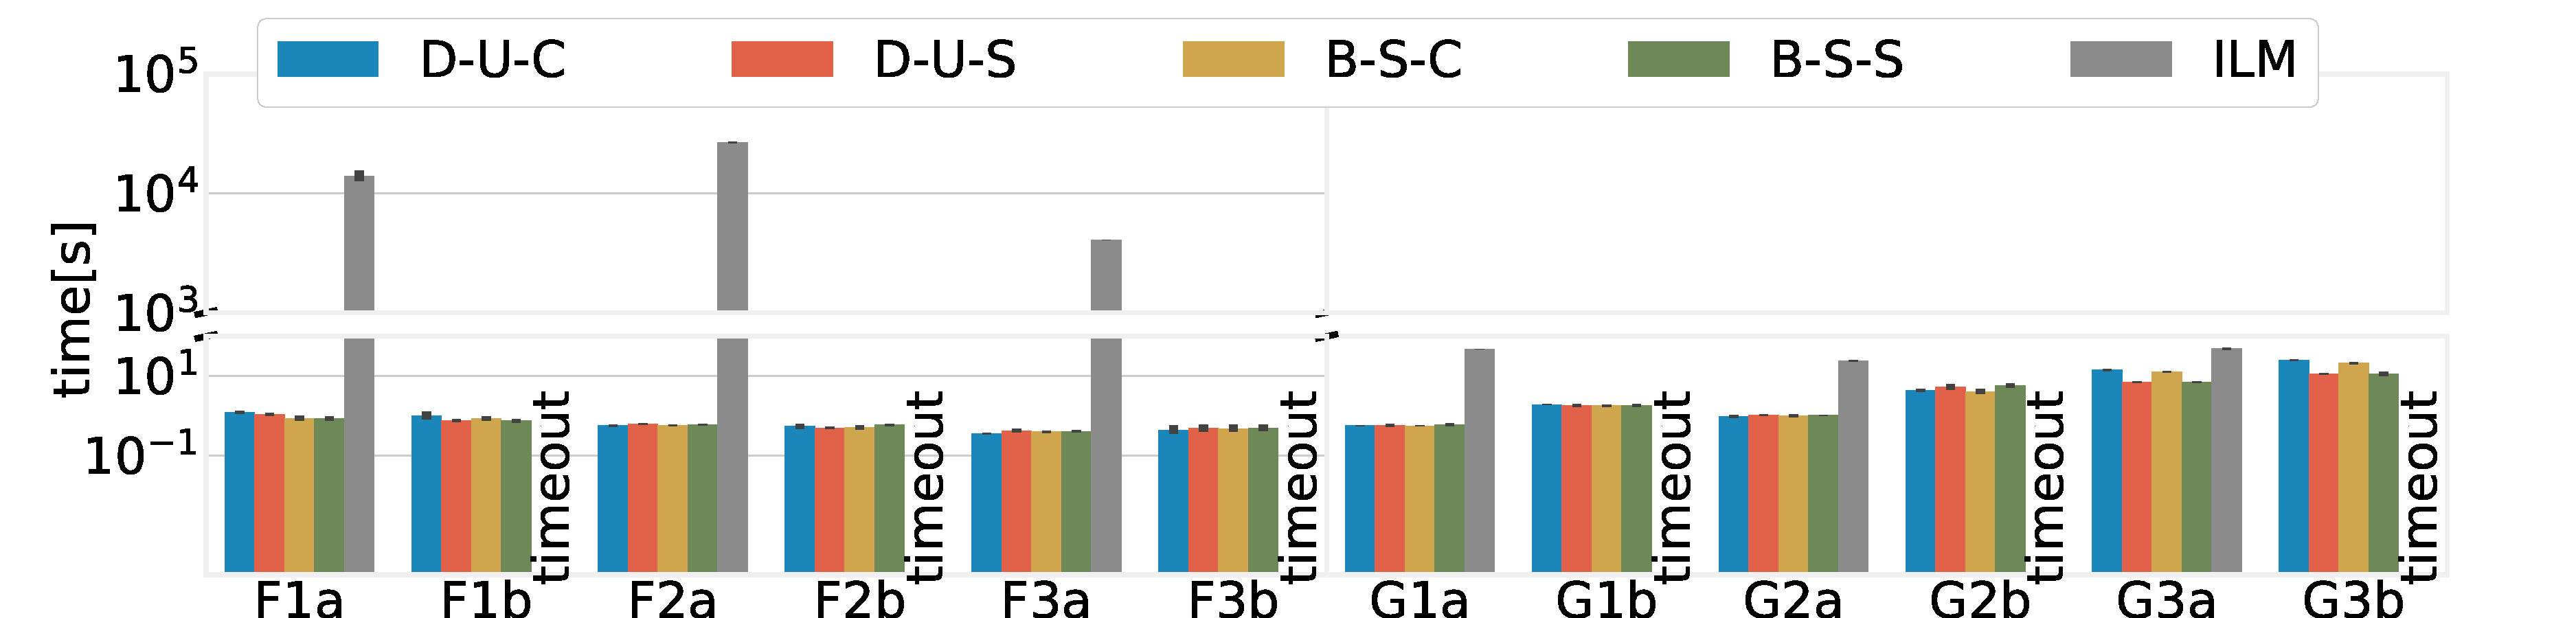
\includegraphics[clip, trim=1em 0em 1em 1em,
		width=1\textwidth]{img/sota_4_broken_new.pdf}
		\vspace{-1.5em}
		\caption{Runtime comparison with the state of the art.}

	\label{fig:sota}
\end{minipage}
\begin{minipage}[c]{0.35\textwidth}
	\vspace{2em}

	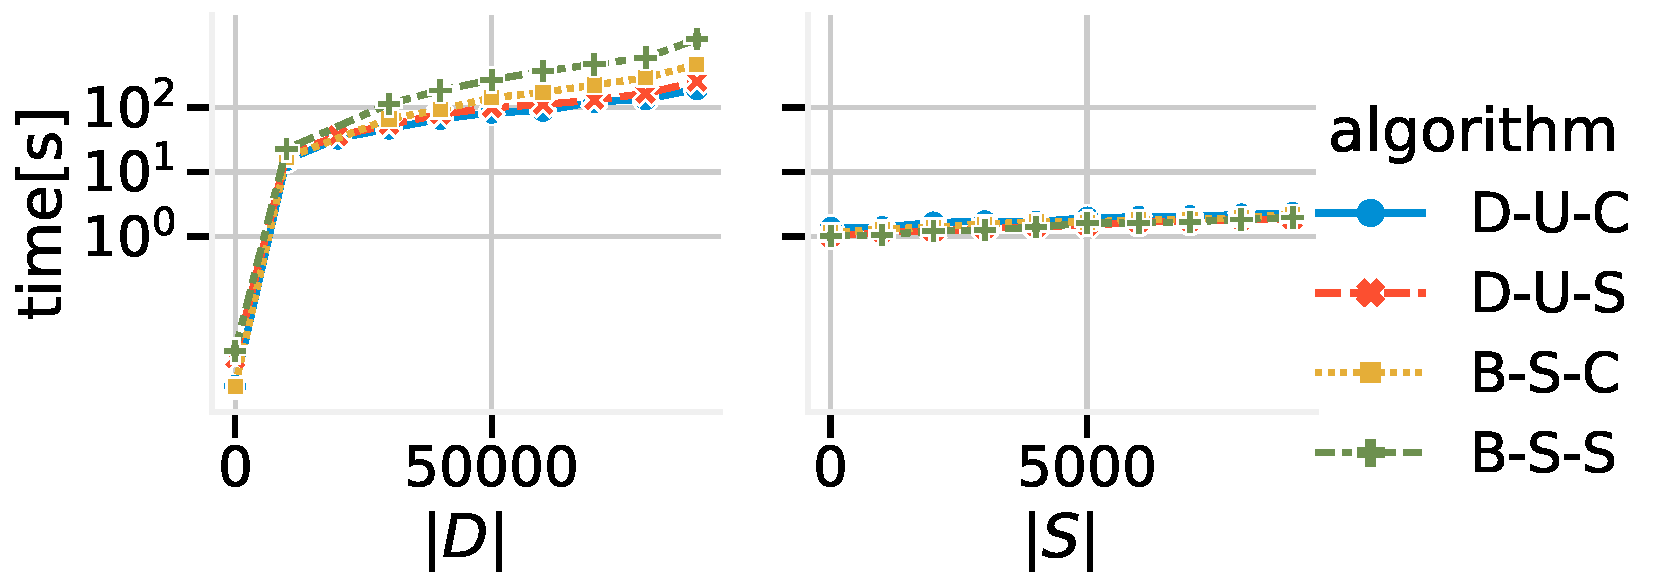
\includegraphics[clip, trim=1em 0em 1em 1em,
	width=1\textwidth]{img/scalability_plots.pdf}
	\vspace{-1.7em}
	\caption{\update{{\normalfont M10\\R1O2\\R3O3}}{Scalability analysis.}}
	\label{fig:scale_plots}
\end{minipage}
\vspace{-1em}
\end{figure*}

\sstitle{Measures} We primarily measure the efficiency of event query
discovery in terms of the algorithms' runtime. We report averages over five
experimental runs, including error bars (mostly negligible).

\sstitle{Environment}
We adopted Python-based implementations of the \sys{} framework and the
IL-Miner.

All experiments were conducted on a server with a Xeon 6354 CPU @3,6GHz and
1TB RAM.
\subsection{State-of-the-Art Comparison}
\label{sec:exp_sota}




First, we compare the runtimes of our algorithms and the
extended IL-Miner, which supports our full query model.

The results in \autoref{fig:sota} show that our algorithms are faster than
the IL-Miner in all cases. For the scenarios based on the finance dataset,
our algorithms are about five orders of magnitude faster. As discussed, we
determined the stream lengths for the $a$ and $b$ scenarios as the
computational limit of the state of the art, i.e., in all $b$ scenarios, the
IL-Miner cannot produce results within 12 hours. The algorithms of the
\sys{} framework enable us to get past this limit in all cases, without a
notable increase in the runtime.

A comparison with the lossy IL-Miner reveals that its improved runtime is traded
for result correctness. The lossy
IL-Miner yields similar runtimes compared to our algorithms, see
\autoref{tab:sota_acc}, yet

it discovers
only a fraction of the queries. With the correct results containing 8
(finance) and 19 (Google) descriptive queries (`Desc'), the lossy IL-Miner
discovers none or only one of them (`Found'), and additionally two and four
queries that are not descriptive (`$\neg$ Desc'). As such, it largely compromises
the result quality not only in terms of descriptiveness, but also in terms of
completeness.



\begin{table}
	\footnotesize
	\caption{Comparison of our algorithms and the lossy IL-Miner.}
	\vspace{-1.2em}
	\label{tab:sota_acc}
	\begin{tabular}{ c c c c c}
\toprule
Datasets & Avg ${}^{\text{Time Lossy ILM}}/_{\text{Time \sys{}}}$ &
{Desc}(riptive) & Found &
$\neg$
{Desc}\\
\midrule
F1b-F3b & 0.42 & 8 & 0 & 4\\
G1b-G3b & 2.9 & 19 & 1 & 2 \\
\bottomrule
\end{tabular}

	\vspace{-1.5em}
\end{table}





\subsection{Scalability Analysis}

\update{M10\\R1O2\\R3O3}{We test the scalability of our algorithms, when
increasing the number of streams and when increasing the minimal
stream length in the database. \autoref{fig:scale_plots} shows that adding
streams yields higher runtimes mainly in beginning, from 2 to 10,000
streams. Afterwards, the trend is close to linear. Differences between the
algorithms are small (D-U-C and D-U-S performing best). Similarly,
increasing the minimal length of a stream does not reveal a particular trend
or differences between the algorithms. These results are in line with our
complexity analysis in \autoref{sec:realizations}, which points to both
properties having a minor impact on the runtime performance. However, our
results confirm the general feasibility of event query discovery with the
\sys{} framework also for larger problem instances.}






\subsection{Sensitivity Analysis}
\label{sec:exp_sensitity}


All of our algorithms show the same worst-case complexity, but incorporate
different design choices. We explore the impact of these choices regarding
properties of stream databases (as introduced in
\autoref{sec:algo_selection}) in a sensitivity analysis.
For the systematically generated stream databases from
\autoref{tab:synt-scenarios}, the results are shown in \autoref{fig:synt_plots}.



For the properties introduced in \autoref{sec:algo_selection}, the results
confirm our hypotheses.
A higher number of attributes (E3) favours algorithms that avoid
merging type and pattern queries: D-U-S and D-U-C outperform B-S-S and
B-S-C, as merging queries becomes expensive with more attributes. Having
more supported attribute values (E4) benefits algorithms that separate the
discovery of type and pattern queries.
B-S-S and B-S-C are more efficient under these conditions, due to the
complexity of unified query handling with a large alphabet.
As for the distribution of supported attribute values (E5), D-U-C and B-S-C
perform better due to reduced merge operations.
Conversely, repeated attribute values (E6) favour D-U-S and B-S-S,
as these approaches minimize the search space for pattern queries.

In sum, our results confirm that the design
choices captured in the \sys{} framework influence the discovery efficiency
as postulated.
The properties of a stream database indeed play a crucial role in
determining which algorithm performs best.

\begin{figure}[t]
	\centering
	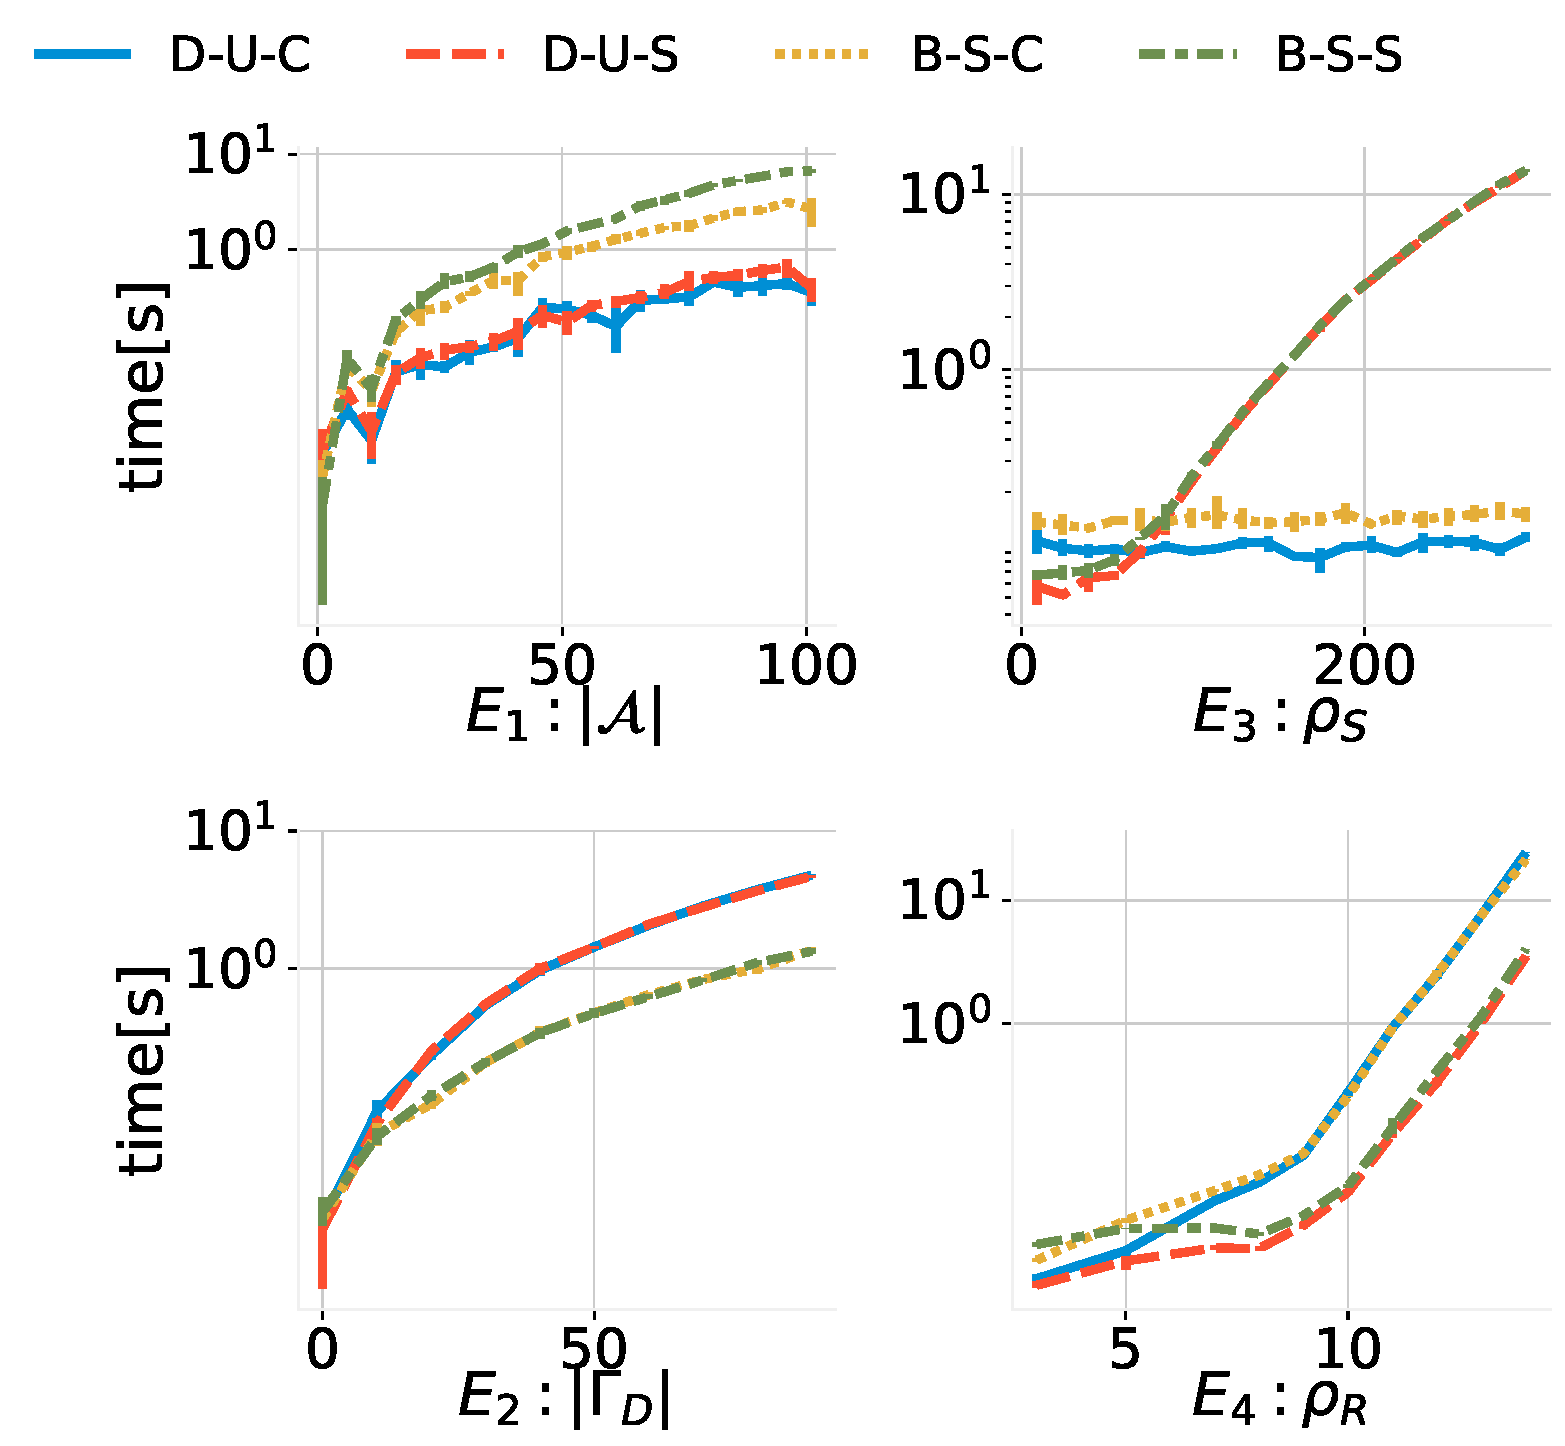
\includegraphics[width=0.75\columnwidth]{img/synt_plots.pdf}
	\vspace{-1em}
	\caption{Sensitivity analysis using synthetic data.}
	\label{fig:synt_plots}
	\vspace{-1.5em}
\end{figure}

\update{M11\\R1O3\\R3O5}{To confirm our results obtained with synthetic data,
we investigated the sensitivity of our algorithms using the Google
dataset.
To obtain the desired variations for each single database property, while
largely keeping the underlying data distributions,
we altered the
existing stream databases $G1, G2, G3$, as follows.
$E_1$: The alphabet $|A|$ was increased by taking one stream and
copying an increasing subset of its events to the remaining streams.
$E_2$: The number of attributes $|\Gamma_D|$ was altered by repeating the
existing
attribute values within an event.
$E_3$: Property $\rho_S$ was increased by copying a number of events
within a stream for a subset of streams within the stream database.
$E_4$: The variation in $\rho_R$ is obtained
selecting an event in each stream and adding it again to the stream.

\autoref{fig:rw-synt} shows that the differences among the algorithms
are less pronounced as for the synthetic data. Yet, there is clear evidence
that the algorithms behave differently for the various properties.
Also, the general trends observed for synthetic data are confirmed.}


\begin{figure*}
	\centering
	\begin{minipage}[c]{0.49\textwidth}
		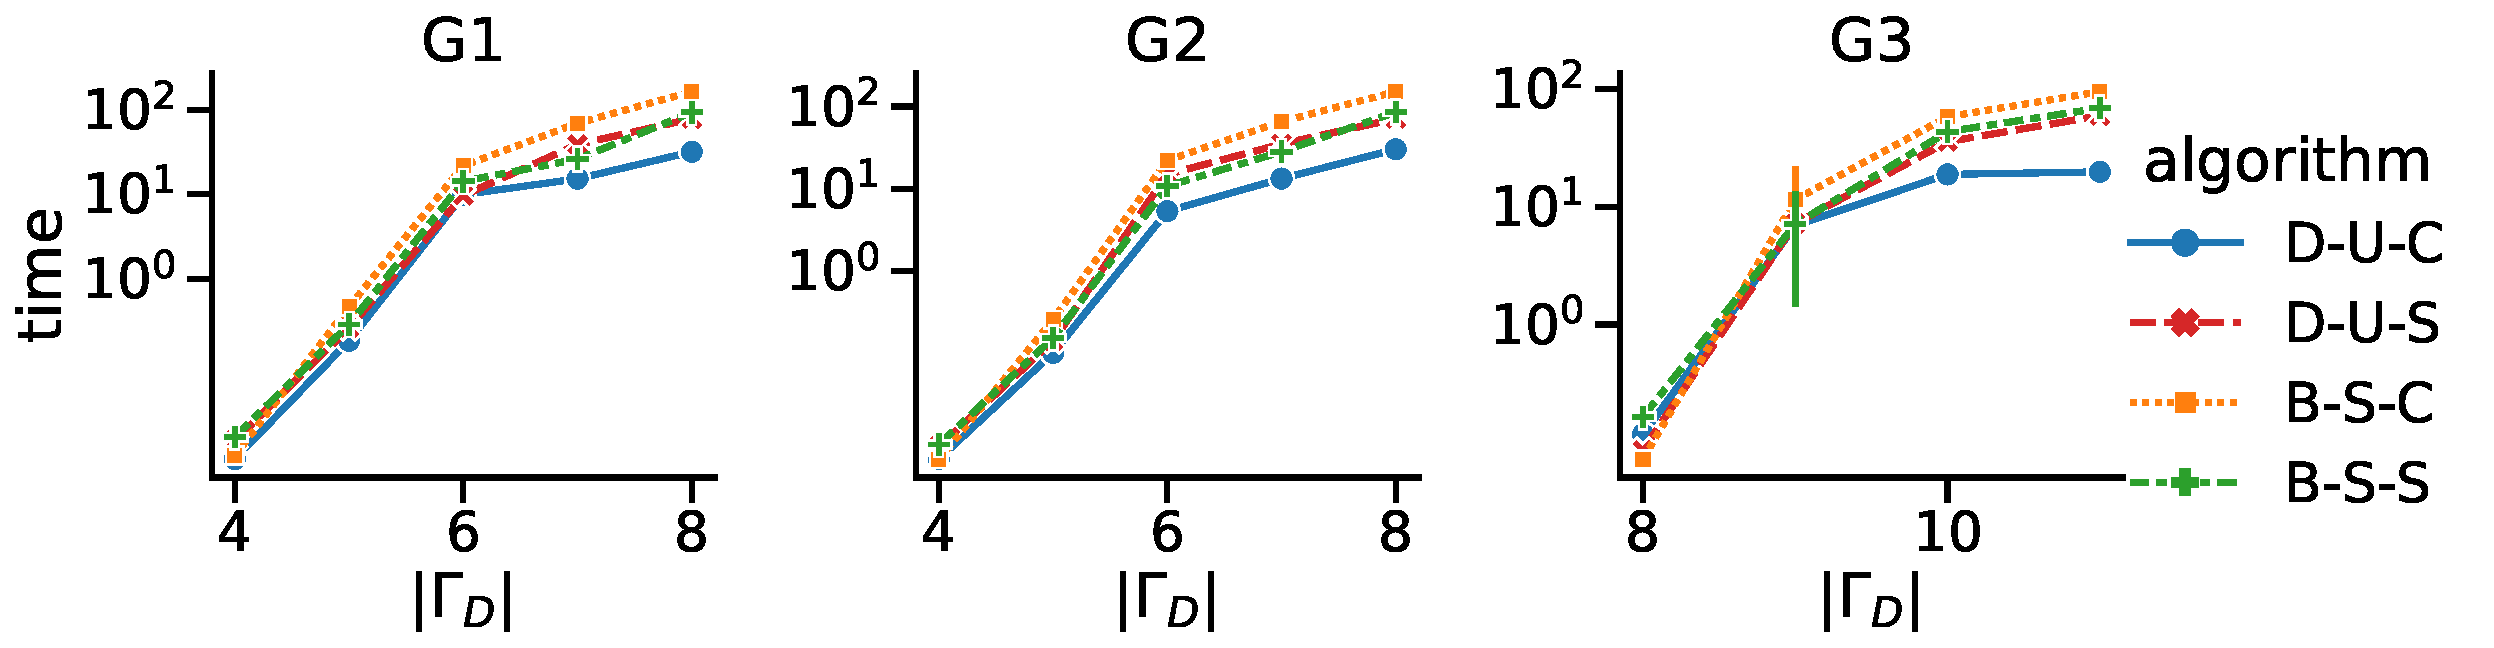
\includegraphics[width=0.95\textwidth]{img/rw_alphabet.pdf}
		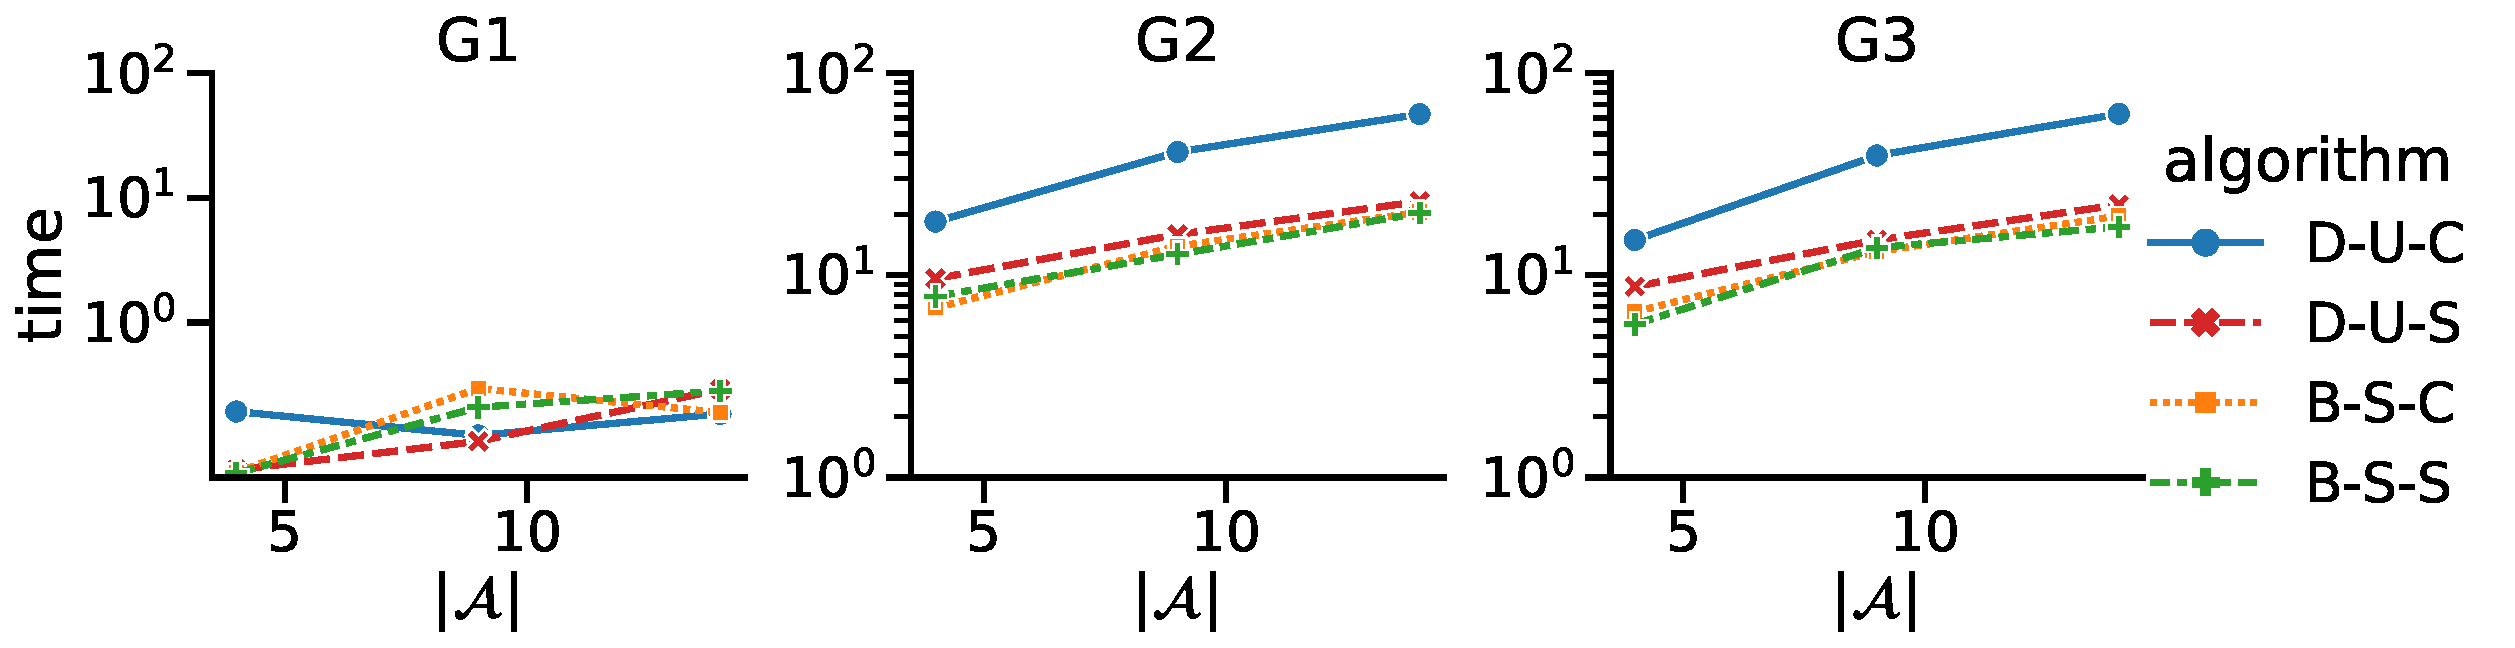
\includegraphics[width=0.95\textwidth]{img/rw_attributes_v2.pdf}
		
\end{minipage}
\begin{minipage}[c]{0.49\textwidth}
	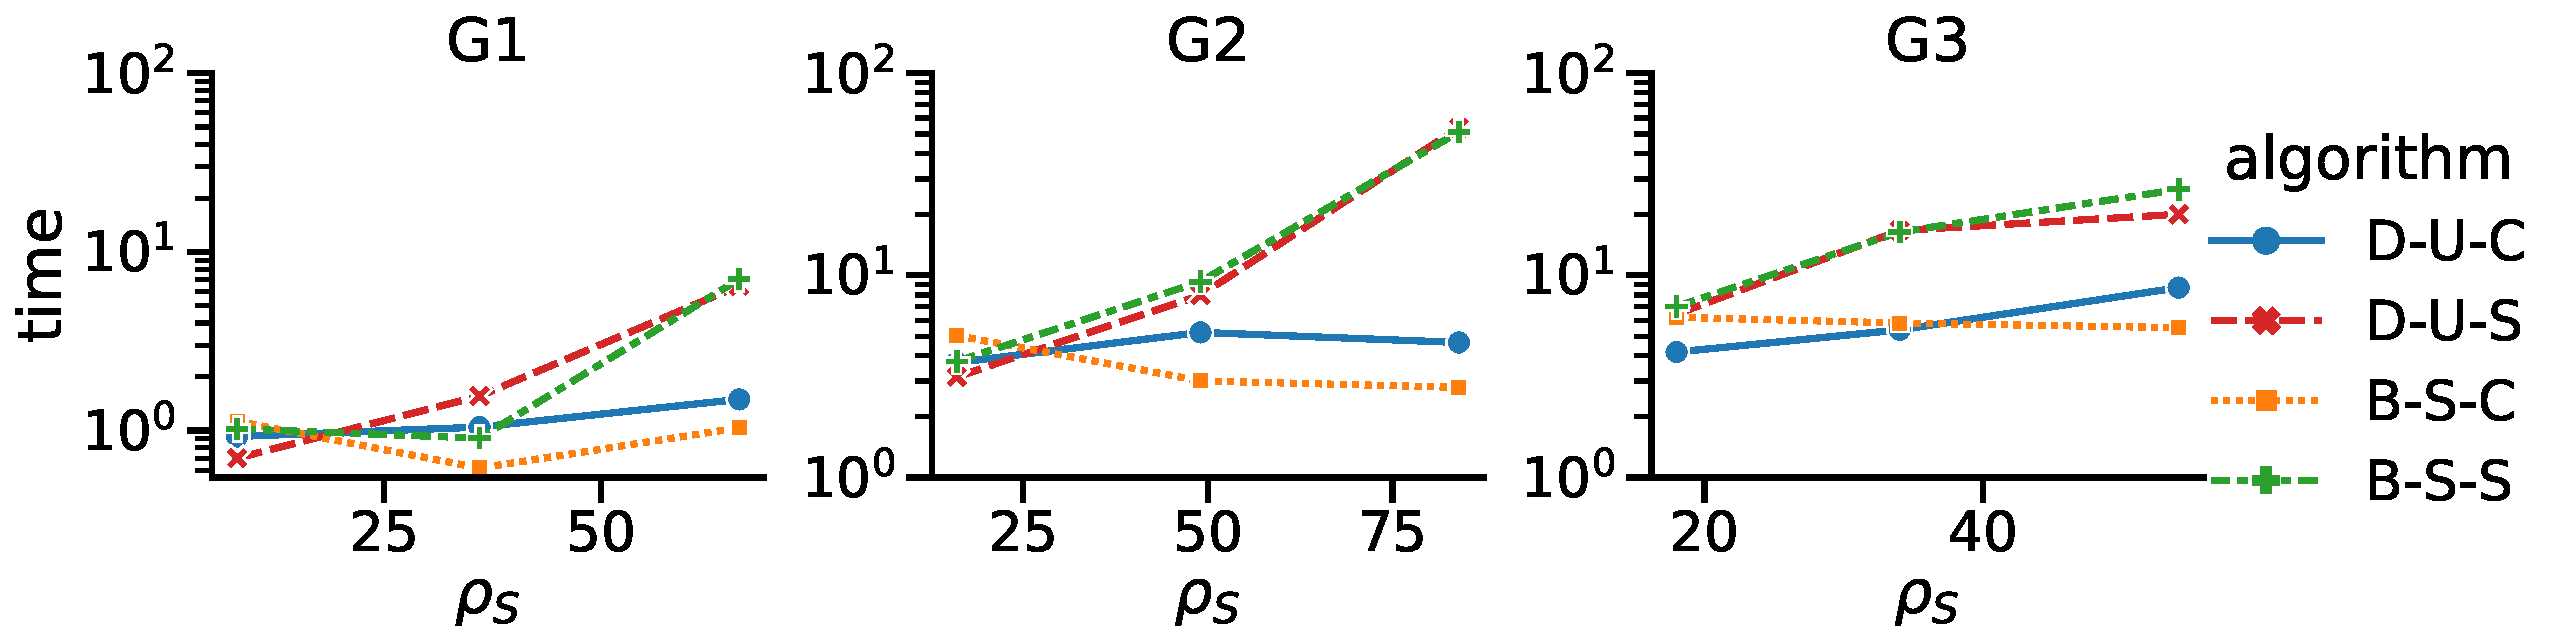
\includegraphics[width=0.95\textwidth]{img/rw_types.pdf}
	
	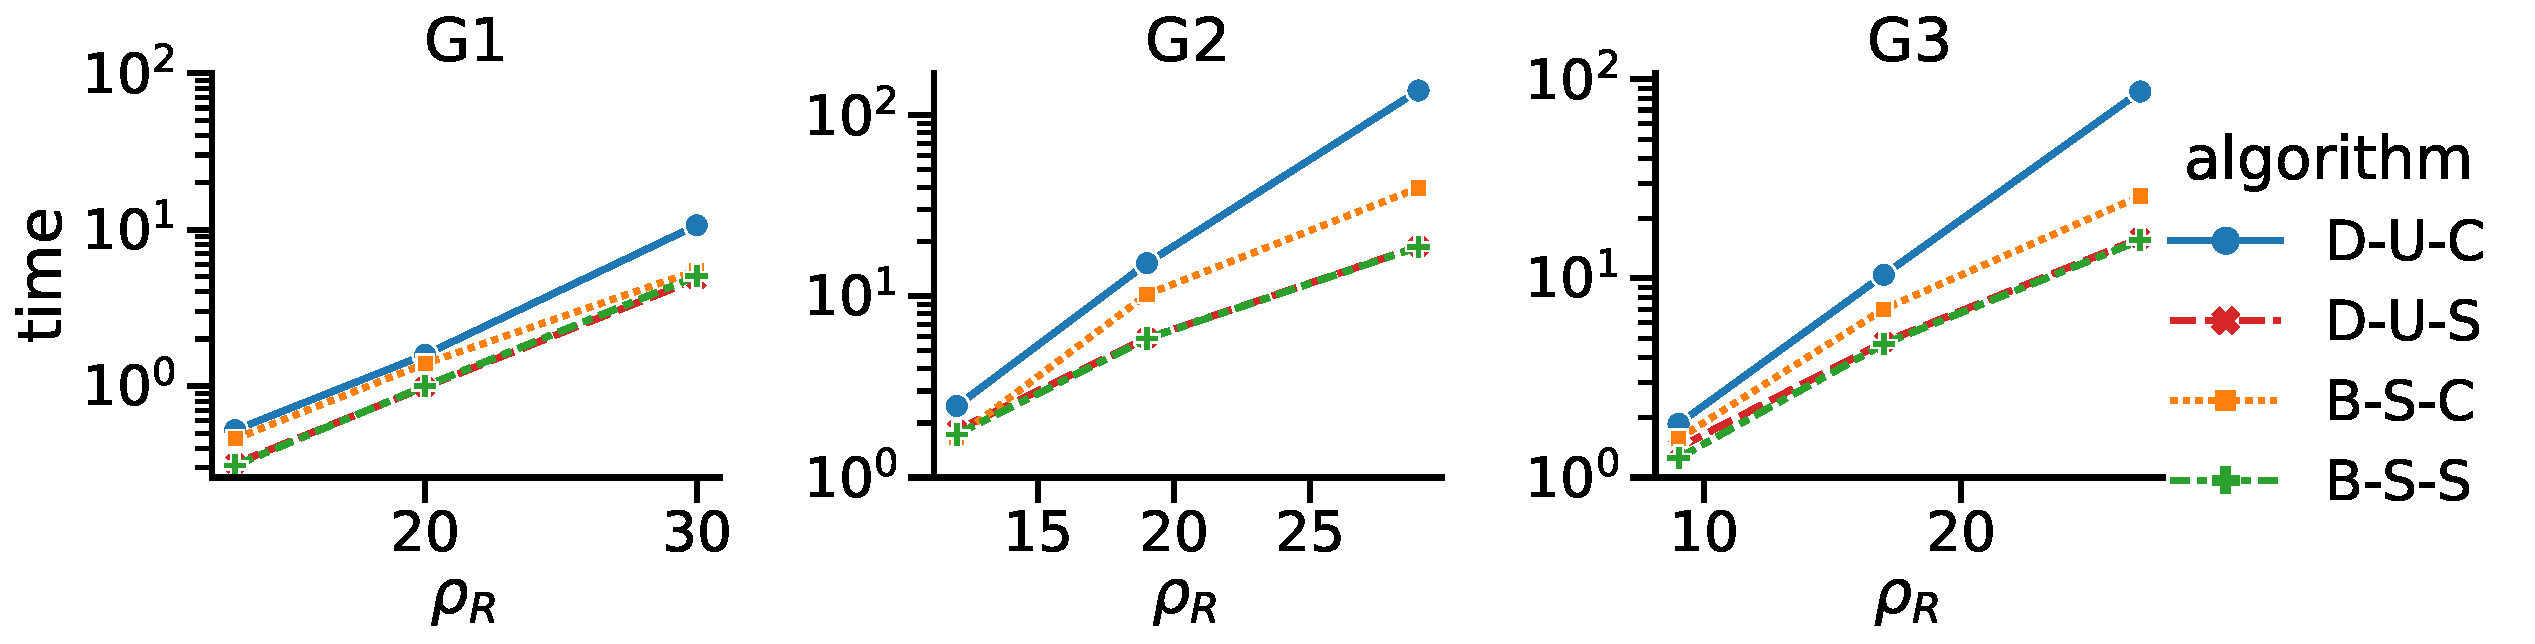
\includegraphics[width=0.95\textwidth]{img/rw_pattern.pdf}
\end{minipage}
\vspace{-1em}
\caption{\update{{\normalfont M11\\R1O3\\R3O5}}{Sensitivity analysis using
the Google
cluster dataset.}}
\label{fig:rw-synt}
\vspace{-.5em}
\end{figure*}


\subsection{Guidance of Query Discovery}
\label{sec:exp_guidance}

\sstitle{Algorithm selection}
Next, we assess whether the above observations enable us to guide the
selection of a discovery algorithm for the real-world data.

From \autoref{tab:char_corr}, we conclude that the
differences in the number of attributes ($|\mathcal{A}|$) and supported
attribute values ($|\Gamma_D|$) are too small to enable any differentiation,
while the results for the repeated attribute values ($\rho_R$) relate to
an inconclusive value range (see \autoref{fig:synt_plots}). Interestingly,
the measure based on the supported attribute values ($\rho_S$) provides
clues on the runtime performance. For $\rho_S=5$, the algorithms
handling attributes separately (D-U-S and B-S-S) perform much better than
those handling them comprehensively. For $\rho_S>10$, the runtimes of our
algorithms show the opposite trend.
Hence, the considered database
properties, assuming that their absolute values provide sufficiently strong
indicators, indeed enable conclusions on the suitability of our algorithms.

\begin{table}[t]
	\footnotesize
	\caption{Correlation of runtime and database properties.}
	\label{tab:char_corr}
	\vspace{-1.5em}
	\begin{tabular}{cccccccc}
\toprule
\multicolumn{4}{c}{Algorithm Runtime} & \multicolumn{4}{c}{Database
Properties} \\
D-U-C & D-U-S & B-S-C & B-S-S & $\rho_R$ & $\rho_S$ & $|\mathcal{A}|$ & $|\Gamma_D|$ \\
\midrule
18.28 & 26.43 & 17.65 & 26.21 & 6 & 11 & 3 & 2 \\
13.50 & 14.95 & 10.52 & 13.34 & 5 & 17 & 3 & 2 \\
0.65 & 1.39 & 0.88 & 1.68 & 9 & 15 & 3 & 6 \\
259.11 & 364.07 & 226.32 & 366.51 & 10 & 12 & 4 & 1 \\
55.43 & 83.84 & 49.32 & 84.51 & 8 & 10 & 4 & 1 \\
533.90 & 172.54 & 488.45 & 172.37 & 8 & 5 & 4 & 1 \\
\bottomrule
\end{tabular}

	\vspace{-1.5em}
\end{table}

\begin{wrapfigure}{r}{0.54\columnwidth}
	\vspace{-1em}
	\centering
	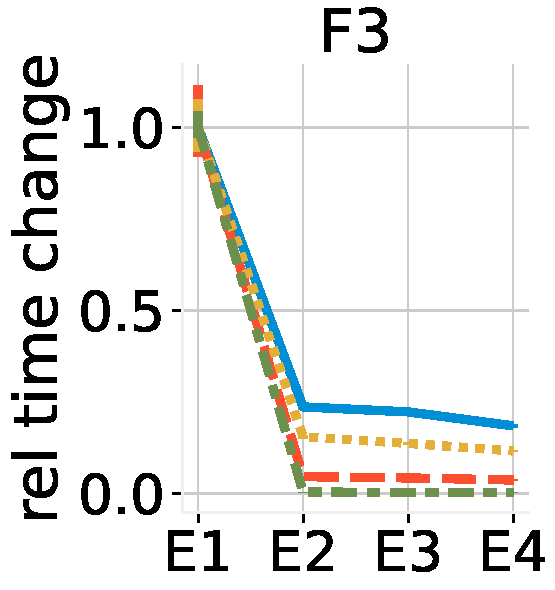
\includegraphics[scale=0.23]{img/exclude-1.pdf}
	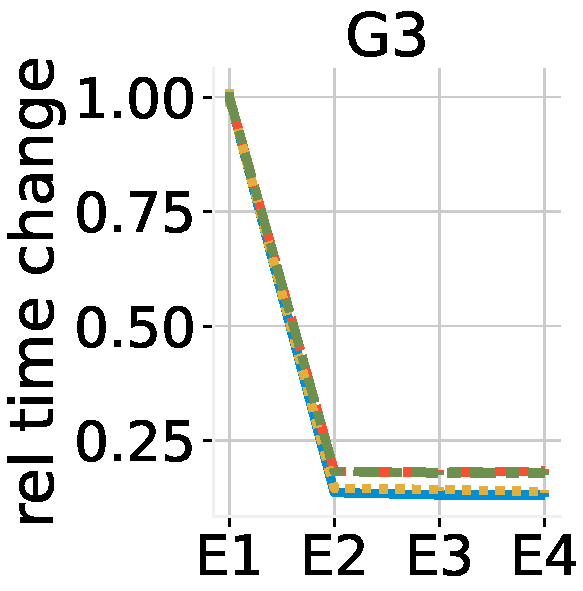
\includegraphics[scale=0.23]{img/exclude-2.pdf}
	\vspace{-1em}
	\caption{Exclusion.}
	\label{fig:exclude}
	
	\vspace{-1em}
\end{wrapfigure}
\sstitle{Feedback mechanisms}
Finally, we tested our mechanisms for feedback on the algorithmic
performance.

First, we assessed whether the exclusion of attribute values may reduce the
discovery runtime.

\autoref{fig:exclude} shows the relative change in
runtimes, when step-wise realizing such an exclusion.
Here, E1 refers to the original database, while for E2-E4, we step-wise
removed the most frequent values of the attribute of the smallest
domain. 
As expected, the runtime  decreases. Since the value
distributions are skewed, excluding the most frequent
value (E2) has the largest effect.


\begin{wrapfigure}{r}{0.54\columnwidth}
	\vspace{-1.5em}
	\centering
	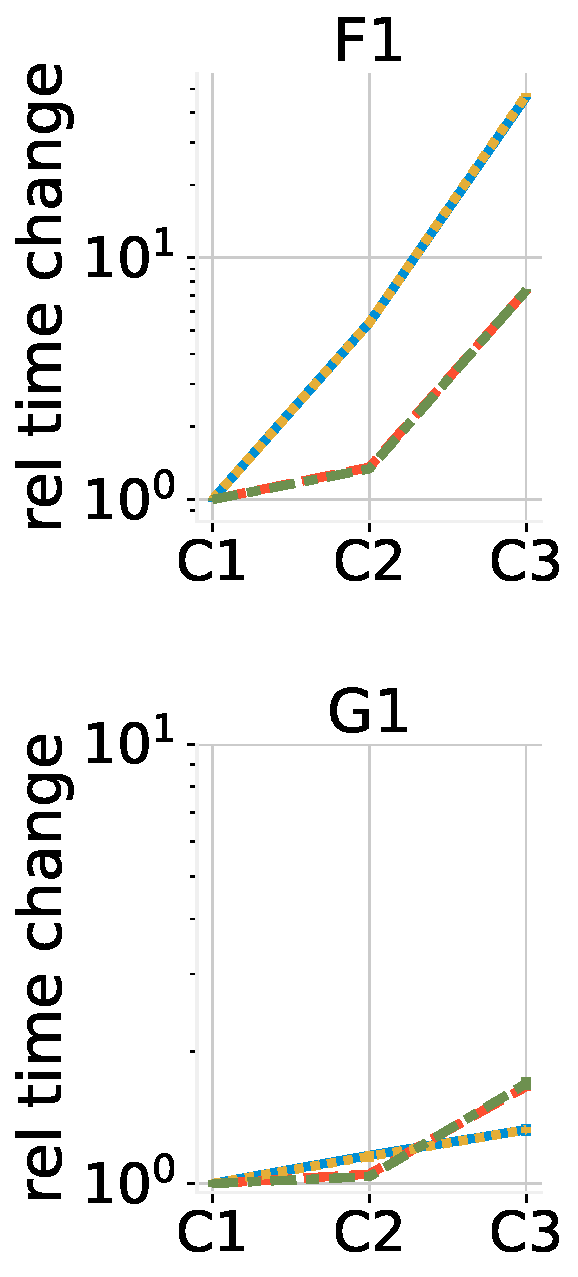
\includegraphics[clip,
	trim=0cm 11.5cm 0cm 0cm, scale=0.23]{img/cluster.pdf}
	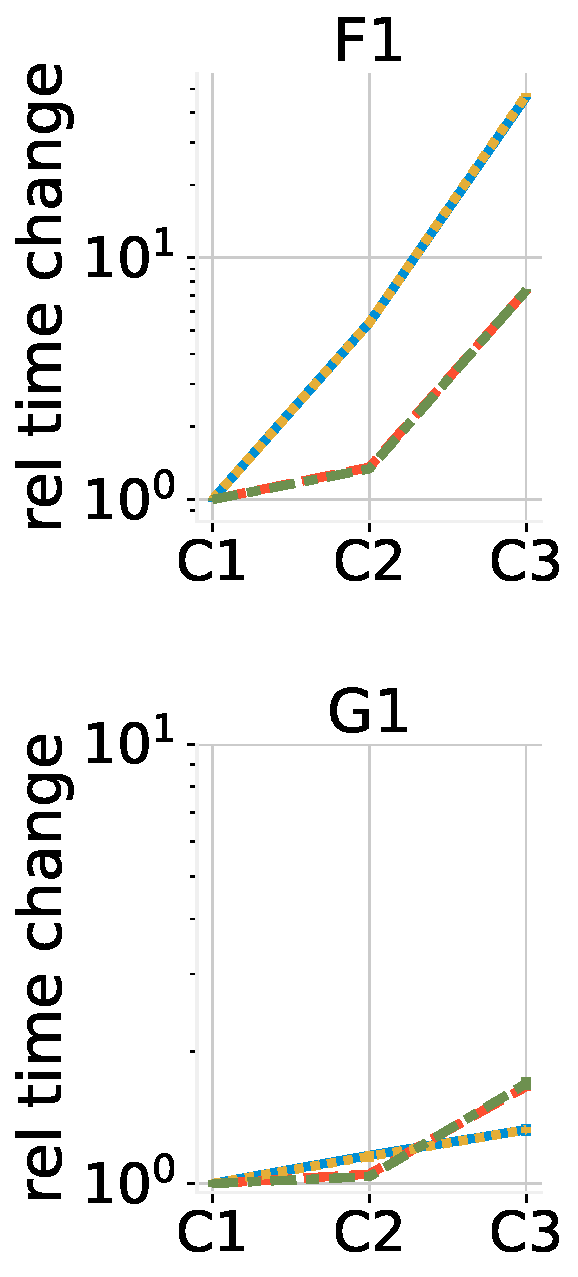
\includegraphics[clip,
	trim=0cm .1cm 0cm 11.5cm, scale=0.23]{img/cluster.pdf}
	\vspace{-2em}
	\caption{Clustering.}
	\label{fig:cluster}
	
	\vspace{-1em}
\end{wrapfigure}
Second, we study the abstraction of clustering of attribute values. C1
denotes the original
dataset without clustering. Then, for the Google dataset, we clustered the
`priority' attribute, as adopted in~\cite{reiss2011google} (C2)
and~\cite{reiss2012towards} (C3). For the finance dataset, we clustered the
`close price' into 100 (C2) or 50 (C3)
equally-sized clusters.
\autoref{fig:cluster} highlights that higher numbers of values
within a cluster increase the runtimes.

However, we
motivated the
abstraction with the desire to increase the result size. For the finance
dataset, we obtain 18 (C1), 30 (C2), and 106 (C3) descriptive queries, while
for the Google dataset, the result includes  202 (C1), 153 (C2), and 298
(C3) queries. We conclude that the expected trend materializes for our data,

However, clustering may also lead to similar descriptive queries
being merged
into one, which may dominate the effect of having more descriptive queries
due to smaller attribute domains.
